\begin{strip}
\centering
\ifteaserdraft
  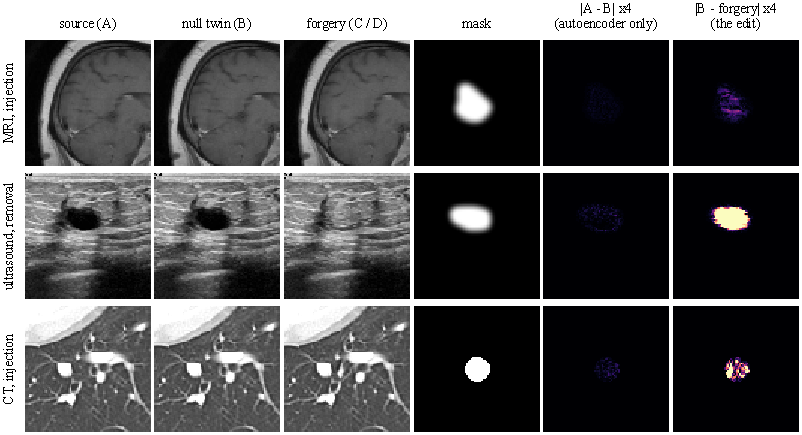
\includegraphics[width=\linewidth]{figures/teaser_draft.pdf}
\else
  \fbox{\parbox[c][1.55in][c]{0.97\linewidth}{\centering\small
  \textbf{[TEASER PLACEHOLDER]}\\[3pt]
  Three lineages (MRI injection, ultrasound removal, CT injection), one row each, cropped around the mask.
  Columns: \emph{source} (A) \textbar{} \emph{null twin} (B: the source round-tripped through the SD autoencoder inside the mask, no edit) \textbar{}
  \emph{forgery} (C or D) \textbar{} \emph{mask} \textbar{} $|$A$-$B$|\times4$ (what the autoencoder alone changed) \textbar{} $|$B$-$forgery$|\times4$ (what the edit changed).\\[3pt]
  Message: the autoencoder change is nearly invisible, the edit is not, yet a standard detector calls both images fake.
  Annotate each image with MedForge-Reasoner's or standard Mesorch's verdict once a per-image score is chosen.\\[3pt]
  A draft built from our own release images is in \texttt{figures/teaser\_draft.pdf}; set \texttt{\textbackslash teaserdrafttrue} in \texttt{macros.tex} to show it.
  No MedForge image may appear (C-UDA licence).}}
\fi
\captionsetup{hypcap=false}
\captionof{figure}{\textbf{One lineage, three images.} The null twin (B) went through the generator's autoencoder exactly as the forgery did but contains no edit; outside the mask, every image is bit-identical to the source.
MedForge-Reasoner flags 0.5\% of untouched scans % src: paper/data/medforge_reasoner_hardlabel.csv (derived from work/e0/out_local/e2/scores_reasoner.parquet)
and 92.5\% of their SD-autoencoder twins as deepfakes (\cref{sec:confound}). % src: paper/data/medforge_reasoner_hardlabel.csv
\TODO{replace placeholder with the final teaser}}
\captionsetup{hypcap=true}
\label{fig:teaser}
\end{strip}
